\documentclass[10pt]{iopart}

\usepackage{graphicx}
\graphicspath{{./figures/}}
%\usepackage[acronym]{glossaries}
\usepackage{acro}
%\newacronym{<++>}{<++>}{<++>}
\newacronym[longplural={metric tons of heavy metal}]{MTHM}{MTHM}{metric ton of heavy metal}
\newacronym{ABM}{ABM}{agent-based modeling}
\newacronym{ACDIS}{ACDIS}{Program in Arms Control \& Domestic and International Security}
\newacronym{ADS}{ADS}{Accelerator-Driven System}
\newacronym{AFCI}{AFCI}{Advanced Fuel Cycles Initiative}
\newacronym{AHTR}{AHTR}{Advanced High Temperature Reactor}
\newacronym{ANDRA}{ANDRA}{Agence Nationale pour la gestion des D\'echets RAdioactifs, the French National Agency for Radioactive Waste Management}
\newacronym{ANL}{ANL}{Argonne National Laboratory}
\newacronym{ANS}{ANS}{American Nuclear Society}
\newacronym{API}{API}{application programming interface}
\newacronym{ARE}{ARE}{Aircraft Reactor Experiment}
\newacronym{ARFC}{ARFC}{Advanced Reactors and Fuel Cycles}
\newacronym{ASME}{ASME}{American Society of Mechanical Engineers}
\newacronym{ASTRID}{ASTRID}{Advanced Sodium Technological Reactor for Industrial Demonstration}
\newacronym{ATWS}{ATWS}{Anticipated Transient Without Scram}
\newacronym{BDBE}{BDBE}{Beyond Design Basis Event}
\newacronym{BIDS}{BIDS}{Berkeley Institute for Data Science}
\newacronym{BWR}{BWR}{Boiling Water Reactor}
\newacronym{CAFCA}{CAFCA}{ Code for Advanced Fuel Cycles Assessment }
\newacronym{CDTN}{CDTN}{Centro de Desenvolvimento da Tecnologia Nuclear}
\newacronym{CEA}{CEA}{Commissariat \`a l'\'Energie Atomique et aux \'Energies Alternatives}
\newacronym{CI}{CI}{continuous integration}
\newacronym{CNEN}{CNEN}{Comiss\~{a}o Nacional de Energia Nuclear}
\newacronym{CNERG}{CNERG}{Computational Nuclear Engineering Research Group}
\newacronym{COSI}{COSI}{Commelini-Sicard}
\newacronym{COTS}{COTS}{commercial, off-the-shelf}
\newacronym{CSNF}{CSNF}{commercial spent nuclear fuel}
\newacronym{CTAH}{CTAHs}{Coiled Tube Air Heaters}
\newacronym{CUBIT}{CUBIT}{CUBIT Geometry and Mesh Generation Toolkit}
\newacronym{CURIE}{CURIE}{Centralized Used Fuel Resource for Information Exchange}
\newacronym{DAG}{DAG}{directed acyclic graph}
\newacronym{DANESS}{DANESS}{Dynamic Analysis of Nuclear Energy System Strategies}
\newacronym{DBE}{DBE}{Design Basis Event}
\newacronym{DESAE}{DESAE}{Dynamic Analysis of Nuclear Energy Systems Strategies}
\newacronym{DHS}{DHS}{Department of Homeland Security}
\newacronym{DOE}{DOE}{Department of Energy}
\newacronym{DRACS}{DRACS}{Direct Reactor Auxiliary Cooling System}
\newacronym{DRE}{DRE}{dynamic resource exchange}
\newacronym{DSNF}{DSNF}{DOE spent nuclear fuel}
\newacronym{DYMOND}{DYMOND}{Dynamic Model of Nuclear Development }
\newacronym{EBS}{EBS}{Engineered Barrier System}
\newacronym{EDF}{EDF}{Électricité de France}
\newacronym{EDZ}{EDZ}{Excavation Disturbed Zone}
\newacronym{EIA}{EIA}{U.S. Energy Information Administration}
\newacronym{EPA}{EPA}{Environmental Protection Agency}
\newacronym{EPR}{EPR}{European Pressurized Reactor}
\newacronym{EP}{EP}{Engineering Physics}
\newacronym{EU}{EU}{European Union}
\newacronym{FCO}{FCO}{Fuel Cycle Options}
\newacronym{FCT}{FCT}{Fuel Cycle Technology}
\newacronym{FEHM}{FEHM}{Finite Element Heat and Mass Transfer}
\newacronym{FEPs}{FEPs}{Features, Events, and Processes}
\newacronym{FHR}{FHR}{Fluoride-Salt-Cooled High-Temperature Reactor}
\newacronym{FLiBe}{FLiBe}{Fluoride-Lithium-Beryllium}
\newacronym{FP}{FP}{Fission Products}
\newacronym{GDSE}{GDSE}{Generic Disposal System Environment}
\newacronym{GDSM}{GDSM}{Generic Disposal System Model}
\newacronym{GENIUSv1}{GENIUSv1}{Global Evaluation of Nuclear Infrastructure Utilization Scenarios, Version 1}
\newacronym{GENIUSv2}{GENIUSv2}{Global Evaluation of Nuclear Infrastructure Utilization Scenarios, Version 2}
\newacronym{GENIUS}{GENIUS}{Global Evaluation of Nuclear Infrastructure Utilization Scenarios}
\newacronym{GPAM}{GPAM}{Generic Performance Assessment Model}
\newacronym{GRSAC}{GRSAC}{Graphite Reactor Severe Accident Code}
\newacronym{GUI}{GUI}{graphical user interface}
\newacronym{HLW}{HLW}{high level waste}
\newacronym{HPC}{HPC}{high-performance computing}
\newacronym{HTC}{HTC}{high-throughput computing}
\newacronym{HTGR}{HTGR}{High Temperature Gas-Cooled Reactor}
\newacronym{IAEA}{IAEA}{International Atomic Energy Agency}
\newacronym{IEMA}{IEMA}{Illinois Emergency Mangament Agency}
\newacronym{IHLRWM}{IHLRWM}{International High Level Radioactive Waste Management}
\newacronym{INL}{INL}{Idaho National Laboratory}
\newacronym{IPRR1}{IRP-R1}{Instituto de Pesquisas Radioativas Reator 1}
\newacronym{IRP}{IRP}{Integrated Research Project}
\newacronym{ISFSI}{ISFSI}{Independent Spent Fuel Storage Installation}
\newacronym{ISRG}{ISRG}{Independent Student Research Group}
\newacronym{JFNK}{JFNK}{Jacobian-Free Newton Krylov}
\newacronym{LANL}{LANL}{Los Alamos National Laboratory}
\newacronym{LBNL}{LBNL}{Lawrence Berkeley National Laboratory}
\newacronym{LCOE}{LCOE}{levelized cost of electricity}
\newacronym{LDRD}{LDRD}{laboratory directed research and development}
\newacronym{LFR}{LFR}{Lead-Cooled Fast Reactor}
\newacronym{LLNL}{LLNL}{Lawrence Livermore National Laboratory}
\newacronym{LMFBR}{LMFBR}{Liquid Metal Fast Breeder Reactor}
\newacronym{LOFC}{LOFC}{Loss of Forced Cooling}
\newacronym{LOHS}{LOHS}{Loss of Heat Sink}
\newacronym{LOLA}{LOLA}{Loss of Large Area}
\newacronym{LP}{LP}{linear program}
\newacronym{LWR}{LWR}{Light Water Reactor}
\newacronym{MAGNOX}{MAGNOX}{Magnesium Alloy Graphie Moderated Gas Cooled Uranium Oxide Reactor}
\newacronym{MA}{MA}{minor actinide}
\newacronym{MCNP}{MCNP}{Monte Carlo N-Particle code}
\newacronym{MILP}{MILP}{mixed-integer linear program}
\newacronym{MIT}{MIT}{the Massachusetts Institute of Technology}
\newacronym{MOAB}{MOAB}{Mesh-Oriented datABase}
\newacronym{MOOSE}{MOOSE}{Multiphysics Object-Oriented Simulation Environment}
\newacronym{MOX}{MOX}{Mixed Oxide Fuel}
\newacronym{MSBR}{MSBR}{Molten Salt Breeder Reactor}
\newacronym{MSRE}{MSRE}{Molten Salt Reactor Experiment}
\newacronym{MSR}{MSR}{Molten Salt Reactor}
\newacronym{MWe}{MWe}{Megawatts electric}
\newacronym{NAGRA}{NAGRA}{National Cooperative for the Disposal of Radioactive Waste}
\newacronym{NEAMS}{NEAMS}{Nuclear Engineering Advanced Modeling and Simulation}
\newacronym{NEUP}{NEUP}{Nuclear Energy University Programs}
\newacronym{NFCSim}{NFCSim}{Nuclear Fuel Cycle Simulator}
\newacronym{NGNP}{NGNP}{Next Generation Nuclear Plant}
\newacronym{NMWPC}{NMWPC}{Nuclear MW Per Capita}
\newacronym{NNSA}{NNSA}{National Nuclear Security Administration}
\newacronym{NPRE}{NPRE}{Department of Nuclear, Plasma, and Radiological Engineering}
\newacronym{NQA1}{NQA-1}{Nuclear Quality Assurance - 1}
\newacronym{NRC}{NRC}{Nuclear Regulatory Commission}
\newacronym{NSF}{NSF}{National Science Foundation}
\newacronym{NSSC}{NSSC}{Nuclear Science and Security Consortium}
\newacronym{NUWASTE}{NUWASTE}{Nuclear Waste Assessment System for Technical Evaluation}
\newacronym{NWF}{NWF}{Nuclear Waste Fund}
\newacronym{NWTRB}{NWTRB}{Nuclear Waste Technical Review Board}
\newacronym{OCRWM}{OCRWM}{Office of Civilian Radioactive Waste Management}
\newacronym{ORION}{ORION}{ORION}
\newacronym{ORNL}{ORNL}{Oak Ridge National Laboratory}
\newacronym{PARCS}{PARCS}{Purdue Advanced Reactor Core Simulator}
\newacronym{PBAHTR}{PB-AHTR}{Pebble Bed Advanced High Temperature Reactor}
\newacronym{PBFHR}{PB-FHR}{Pebble-Bed Fluoride-Salt-Cooled High-Temperature Reactor}
\newacronym{PEI}{PEI}{Peak Environmental Impact}
\newacronym{PHWR}{PHWR}{Pressurized Heavy Water Reactor}
\newacronym{PH}{PRONGHORN}{PRONGHORN}
\newacronym{PRIS}{PRIS}{Power Reactor Information System}
\newacronym{PRKE}{PRKE}{Point Reactor Kinetics Equations}
\newacronym{PSPG}{PSPG}{Pressure-Stabilizing/Petrov-Galerkin}
\newacronym{PWAR}{PWAR}{Pratt and Whitney Aircraft Reactor}
\newacronym{PWR}{PWR}{Pressurized Water Reactor}
\newacronym{PyNE}{PyNE}{Python toolkit for Nuclear Engineering}
\newacronym{PyRK}{PyRK}{Python for Reactor Kinetics}
\newacronym{QA}{QA}{quality assurance}
\newacronym{RDD}{RD\&D}{Research Development and Demonstration}
\newacronym{RD}{R\&D}{Research and Development}
\newacronym{RELAP}{RELAP}{Reactor Excursion and Leak Analysis Program}
\newacronym{RIA}{RIA}{Reactivity Insertion Accident}
\newacronym{RIF}{RIF}{Region-Institution-Facility}
\newacronym{SFR}{SFR}{Sodium-Cooled Fast Reactor}
\newacronym{SINDAG}{SINDA{\textbackslash}G}{Systems Improved Numerical Differencing Analyzer $\backslash$ Gaski}
\newacronym{SKB}{SKB}{Svensk K\"{a}rnbr\"{a}nslehantering AB}
\newacronym{SNF}{SNF}{spent nuclear fuel}
\newacronym{SNL}{SNL}{Sandia National Laboratory}
\newacronym{STC}{STC}{specific temperature change}
\newacronym{SUPG}{SUPG}{Streamline-Upwind/Petrov-Galerkin}
\newacronym{SWF}{SWF}{Separations and Waste Forms}
\newacronym{SWU}{SWU}{Separative Work Unit}
\newacronym{TRIGA}{TRIGA}{Training Research Isotope General Atomic}
\newacronym{TRISO}{TRISO}{Tristructural Isotropic}
\newacronym{TSM}{TSM}{Total System Model}
\newacronym{TSPA}{TSPA}{Total System Performance Assessment for the Yucca Mountain License Application}
\newacronym{ThOX}{ThOX}{thorium oxide}
\newacronym{UFD}{UFD}{Used Fuel Disposition}
\newacronym{UML}{UML}{Unified Modeling Language}
\newacronym{UNF}{UNF}{Used Nuclear Fuel}
\newacronym{UOX}{UOX}{Uranium Oxide Fuel}
\newacronym{UQ}{UQ}{uncertainty quantification}
\newacronym{US}{US}{United States}
\newacronym{UW}{UW}{University of Wisconsin}
\newacronym{VISION}{VISION}{the Verifiable Fuel Cycle Simulation Model}
\newacronym{VVER}{VVER}{Voda-Vodyanoi Energetichesky Reaktor (Russian Pressurized Water Reactor)}
\newacronym{VV}{V\&V}{verification and validation}
\newacronym{WIPP}{WIPP}{Waste Isolation Pilot Plant}
\newacronym{YMR}{YMR}{Yucca Mountain Repository Site}

% \usepackage[numbers]{natbib}
\usepackage{cite}
\usepackage{tabularx}
\usepackage{float}


\begin{document}

\title[Minimizing heatwave risk through an equitable distribution of solar panels]{Minimizing
heatwave risk through an equitable distribution of solar panels}

 \author{
 Samuel G. Dotson$^1$$^*$,
 Shannon R. Anderson$^2$,
 Alankrita Sahay$^3$,
 Pranjali Borse$^3$,
 Charumeghana Samantula$^3$
 }

 \address{ $^1$ Department of Nuclear, Plasma, and Radiological Engineering,
 University of Illinois Urbana-Champaign, Urbana IL, United States}
  \address{ $^2$ Department of  Natural Resources and Environmental Sciences,
 University of Illinois Urbana-Champaign, Urbana IL, United States}
  \address{ $^3$ Department of Civil and Environmental Engineering,
 University of Illinois Urbana-Champaign, Urbana IL, United States}
 \address{$^*$ Author to whom correspondence should be addressed}

 \ead{sgd2@illinois.edu}

 \begin{indented}
 \vspace{10pt}
 \item[]May 2022
 \end{indented}

 \begin{abstract}
Heat wave frequency and severity are increasing due to anthropogenic climate change.
Cities face higher consequences from heat waves because of the \ac{uhi} effect.
Rooftop solar panels are one method to mitigate \ac{uhi} and improve the adaptive
capacity of urban residents by lowering the cost of energy for low-income households.
This work uses a set of socioeconomic data, such as age, energy burden, population
density, and isolation, along with satellite temperature data, to identify regions
of high heat wave risk in Chicago so those regions may be prioritized for solar
panel subsidies from the state of Illinois. After curation, the data were clustered
using hierarchical clustering. The results of this process show improvements over
current prioritization schemes from the \ac{epa} \ac{ejscreen}. 
 \end{abstract}

 \vspace{2pc}
\noindent{\it Keywords}: solar, heatwave, equity, energy justice, policy

%\ioptwocol
\acresetall

\section{Introduction}
\section{Introduction}

This is the introduction section. For consistency, use the
\texttt{glossaries} package for acronyms such as ``\gls{SFR}".
This automatically populates the glossaries list and abbreviates future
mentions of ``\gls{SFR}".

All tables and figures must be referenced to in the text.
Use the BibTeX package to manage your paper references and bibliography
\cite{huff_extensions_2014}.


\section{Literature Review}
The \ac{uhi} effect, where urban areas tend to be warmer than their surroundings,
is among the most well studied phenomena, often using remote sensing technology and land
surface temperature data \cite{almeida_study_2021, cotlier_extreme_2022}.
Some studies evaluated \ac{uhi} intensity for particular cities by incorporating
data about urban features such as albedo, building height, and vegetation
\cite{sangiorgio_development_2020,abulibdeh_analysis_2021} along with urbanization
trends \cite{li_how_2021}. Other work in the literature examined \ac{uhi} along
a socio-economic axis. Chakraborty et al. \cite{chakraborty_disproportionately_2019}
used satellite and census data for multiple cities and found that \ac{uhi}
disproportionately affects low-income residents in most places, including Chicago,
and suggest that \ac{uhi} mitigation should benefit demographic groups that experience
greater \ac{uhi} intensity. Hsu et al. \cite{hsu_disproportionate_2021} also
found that race and income level were correlated with greater \ac{uhi} intensity.

Strategies to mitigate \ac{uhi} typically interrupt the heat storage process that
drives \ac{uhi}, where
low albedo surfaces such as pavement and rooftops absorb and trap heat. Green roofs
are a popular method to reduce \ac{uhi} by reducing heat storage and increasing
the energy from latent heat rather than sensible heat \cite{zhang_effectiveness_2017}.
Similar to green roofs, several studies determined that increasing the urban
tree canopy is an effective way to reduce \ac{uhi} by reducing heat storage in
surfaces, but also by providing shade \cite{middel_urban_2015,
loughner_roles_2012, mcdonald_tree_2021, marando_urban_2022, schwaab_role_2021}.
``Cool'' roofs reduce \ac{uhi} by increasing the albedo of rooftop surfaces and
decreasing the amount of radiation that gets absorbed \cite{zhang_effectiveness_2017,
salamanca_citywide_2016, middel_urban_2015}. Lastly, rooftop solar panels are also
found to mitigate \ac{uhi} effects at night due to boundary
layer structure and by reducing energy requirements for cooling \cite{masson_solar_2014,
sailor_photovoltaics_2021, salamanca_citywide_2016}. However, the primary
function of solar panels is to improve adaptive capacity by generating energy
for cooling \cite{masson_solar_2014}.

As with \ac{uhi} intensity, the literature also indicates that \ac{uhi} mitigation
efforts disproportionately benefit wealthier residents. McDonald et al. reported
that high-income areas had nearly twice the tree canopy of neighboring low-income
regions \cite{mcdonald_tree_2021}. Further, efforts to mitigate \ac{uhi} with
vegetation may lead to gentrification, thereby excluding the intended beneficiaries
\cite{chakraborty_disproportionately_2019}. Solar panel adoption has also developed
along socio-economic lines. Vaishnav et al. \cite{vaishnav_was_2017} showed that
subsidies for rooftop solar panels favored the affluent. Reames et al.
\cite{reames_distributional_2020} identified that the greatest solar panel
penetration was found in areas with the greatest income, although it remained
quite low compared with other cities. The researchers also indicate that lack
of information contributes to these disparities \cite{vaishnav_was_2017,reames_distributional_2020}.
Illinois' Solar for All campaign sought to prioritize low-income areas using a
tool called the \ac{ejscreen} from the \ac{epa} \cite{us_epa_ejscreen_2014}. Another
tool that identifies climate justice areas is the \ac{cejst}
\cite{council_on_environmental_quality_climate_nodate}. However, neither of these
tools incorporate temperature data nor \ac{uhi} effects, thereby limiting their
effectiveness at targeting areas facing heat wave risk.

In the present work, we use the hazard-exposure-vulnerability framework for
risk established by \ac{ipcc} in 2018 \cite{viner_understanding_2020}. This
framework is useful for understanding the different factors that contribute to
risk. Hazards are the climate events that can produce adverse outcomes. Examples
include flooding, hurricanes, and heat waves. Our work focuses on the latter.
Exposure implies the presence of people. People are not at risk from a hazard if
they are not present. Regions with different population densities have different
levels of exposure. Further, cities have a higher exposure to heat waves due to
\ac{uhi}. Lastly, vulnerability describes susceptibility and adaptive capacity to
particular hazards. This includes socio-economic factors such as race, income,
and age. Adaptive capacity reduces exposure or vulnerabilities while mitigation
efforts minimize the hazard itself.

Lower income is associated with greater \ac{uhi} and therefore
both a greater exposure to heat waves with less adaptive capacity. However, income
is one of many factors that contribute to heat wave risk. Maragno et al.
\cite{maragno_mapping_2020} mapped heat stress risk by adapting the
hazard-exposure-vulnerability framework and included age as a demographic vulnerability
along with landuse for different types of buildings. There are other
socioeconomic factors that contribute to heat wave risk, such as crime rate,
educational attainment, access to cooling centers, and housing characteristics
\cite{klinenberg_heat_2003,gronlund_racial_2014} that Maragno et al. do not include.

Several works mapped regions with the highest \ac{uhi} \cite{almeida_study_2021},
identified disparities in \ac{uhi} \cite{chakraborty_disproportionately_2019} and
its mitigation \cite{reames_distributional_2020, mcdonald_tree_2021}. At least one
study applied the hazard-exposure-vulnerability framework in a heat wave risk
assessment \cite{maragno_mapping_2020}. However, there is no existing literature
that prescribes a methodology for efficient allocation of rooftop solar panels.
The present work fills that gap by collecting satellite and socio-economic data
to identify areas of high heat wave risk that accounts for disparities in
exposure and adaptive capacity.


% \begin{itemize}
%   \item What studies have mapped uhi?
%   \item What papers have looked at uhi and class?
%   \item What papers have looked at uhi mitigation strategies?
%   \item What are the most frequent mitigation strategies (green+white roofs)
%   \item What papers have looked at the solar panel distribution?
%   \item What are the social aspects of solar panel distribution?
%   \item How have solar panels been distributed previously? (Introduce CEJST \& EJSCREEN)
%   \item What gap in the literature is this work specifically filling?
%   \item How are we defining risk? solar panels may worsen the hazard since they have a low albedo.
% \end{itemize}
%
%
%
%
% Various studies have addressed heat wave problem and distribution of solar panels separately till now. An assessment by means of Land Surface Temperature using remote sensing technology \cite{cotlier_extreme_2022}, the mapping of heat stress by crowdsourcing geospatial data and high spatial resolution data and evaluation of socioeconomic characteristics \cite{maragno_mapping_2020}, quantifying synergies between Urban Heat Island effect and heatwaves in urban areas \cite{founda_synergies_2017}  are some of the studies addressing heatwave problem. While these studies mainly discuss about the spatial distribution of heat stress, others have also addressed its implications to the society by assessing socio-economic vulnerability and risk. One of the study\cite{maragno_mapping_2020} has developed sensitivity, adaptive capacity, vulnerability, exposure, and risk indicators and tested the framework on urban area concluding that vulnerability and risk levels differ with changing locational characteristics within the same urban area and hence the high resolution spatial dataset serves a great importance to plan necessary adaptation strategies. This study served as a foreground to choose the high resolution datasets in our study. Our study area is Chicago city which is an highly urbanized area with varying locational characteristics. We reviewed few studies related to Chicago heatwaves. The study by Bernice Ackerman  has addressed the effect of Lake Michigan on temperature of its surrounding area and the effect of green cover. It was helpful in identifying the crucial indicators like green cover and presence of water bodies which help surrounding areas to stay relatively cooler and hence could serve as good adaptive capacity indicators.
%
% Prior research has shown works that study the distributional disparities in residential rooftop solar potential in four major cities in Chicago and a few other cities \cite{reames_distributional_2020}. The study found that the highest rooftop potential in Chicago was in census tracts with higher percentages of \ac{lmi} households. The \ac{lmi} households represented 51\% of solar suitable households in Chicago. However, the lower penetration of solar \ac{lmi} communities substantially decreases the overall attainment of renewable energy and energy equity goals in Chicago.  DeepSolar, a machine learning framework that efficiently constructs a solar deployment dataset for the United States has found that the solar deployment density is strongly correlated and decreases with the Gini index, a measure of income inequality \cite{yu_deepsolar_2018}. This points out how socio-economic inequality causes disparities in solar distribution. Most states across the United States have developed one or more policies to incentivize distributed solar PV investments. Many states have adopted various additional financial incentives to encourage and support the deployment of customer-owned distributed solar energy systems \cite{pitt_assessing_2015}. These policies and incentives are similar to Illinois Shine and Solar for All programs in Illinois which the current study focuses on.
% However, it has also been shown that the distribution of low-carbon technology subsidies and their associated benefits can be highly uneven across socioeconomic groups, revealing a persistent inequality issue. The high income community usually have the resources and knowledge required to avail the benefits of such subsidies and hence tend to be more benefited than their low income counterparts \cite{stewart_all_2021}. This escalates the need for equitable distribution of the solar incentives across different socioeconomic communities. Hence, this study aims to find the ‘high risk’ areas in Chicago and help facilitate equitable distribution of solar panels through the Illinois Shine and Solar for all programs.


\section{Methods and Data}
\label{section:methods_data}
\section{Methodology}
This is the methodology section.

\pagebreak
\subsection{Subsection}

\begin{figure}[h]
        \centering
\begin{tikzpicture}[node distance=1.5cm]
\node (start) [object] {Start};
\node (step1) [process, below of=start] {Step 1};
\node (intermediate) [object, below of=step1] {Intermediate};
\node (step2) [process, below of=intermediate] {Step 2};
\node (end) [object, below of=step2]{End};

\draw [arrow] (start) -- (step1); 
\draw [arrow] (step1) -- (intermediate);
\draw [arrow] (intermediate) -- (step2); 
\draw [arrow] (step2) -- (end);
\end{tikzpicture}
\caption{A caption for the flowchart.}
\label{fig:comp}
\end{figure}


\section{Results}
\label{section:results}
After clustering the data with a hierarchical clustering algorithm, we developed
a map of the most similar regions according to their cluster. Figure \ref{fig:clustering}
shows these regions. The colors and numbers in Figure \ref{fig:clustering} simply
identify the cluster and do not correspond to heat wave risk nor priority.

\begin{figure}[H]
    \begin{center}
      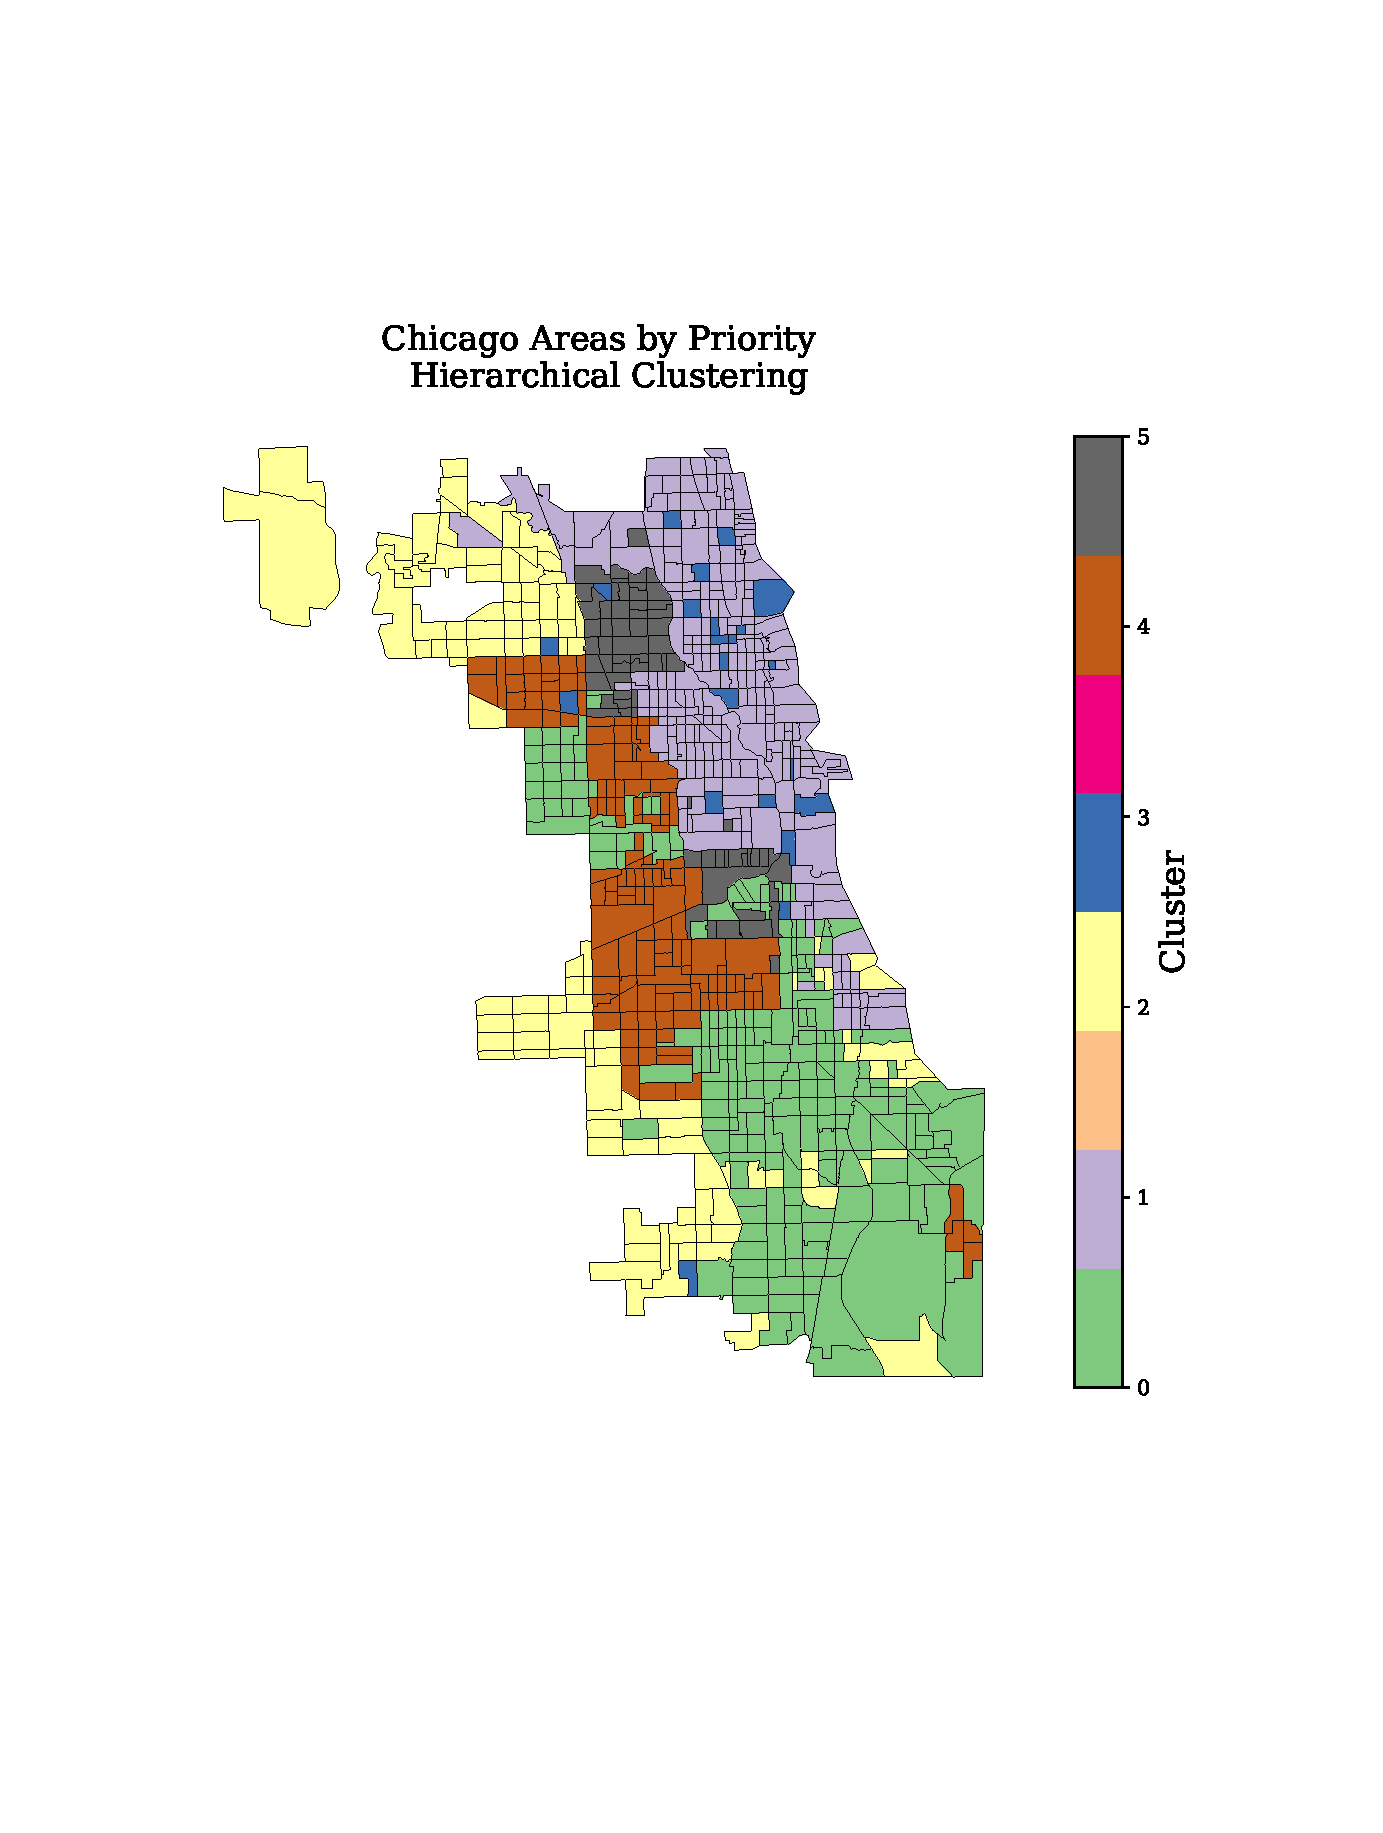
\includegraphics[trim=0 120 0 120, clip, width=\columnwidth]{clustering}
      % \vspace*{-3cm}
      \caption{The map of Chicago clusters. The numbers correspond to the order
      in which the algorithm created the groups and not the heatwave risk.}
      \label{fig:clustering}
    \end{center}
\end{figure}

Figure \ref{fig:cluster_compare} compares the mean vector of each cluster. The
colors and group numbers match the colors and group numbers from Figure
\ref{fig:clustering}.

\begin{figure}[H]
    \begin{center}
      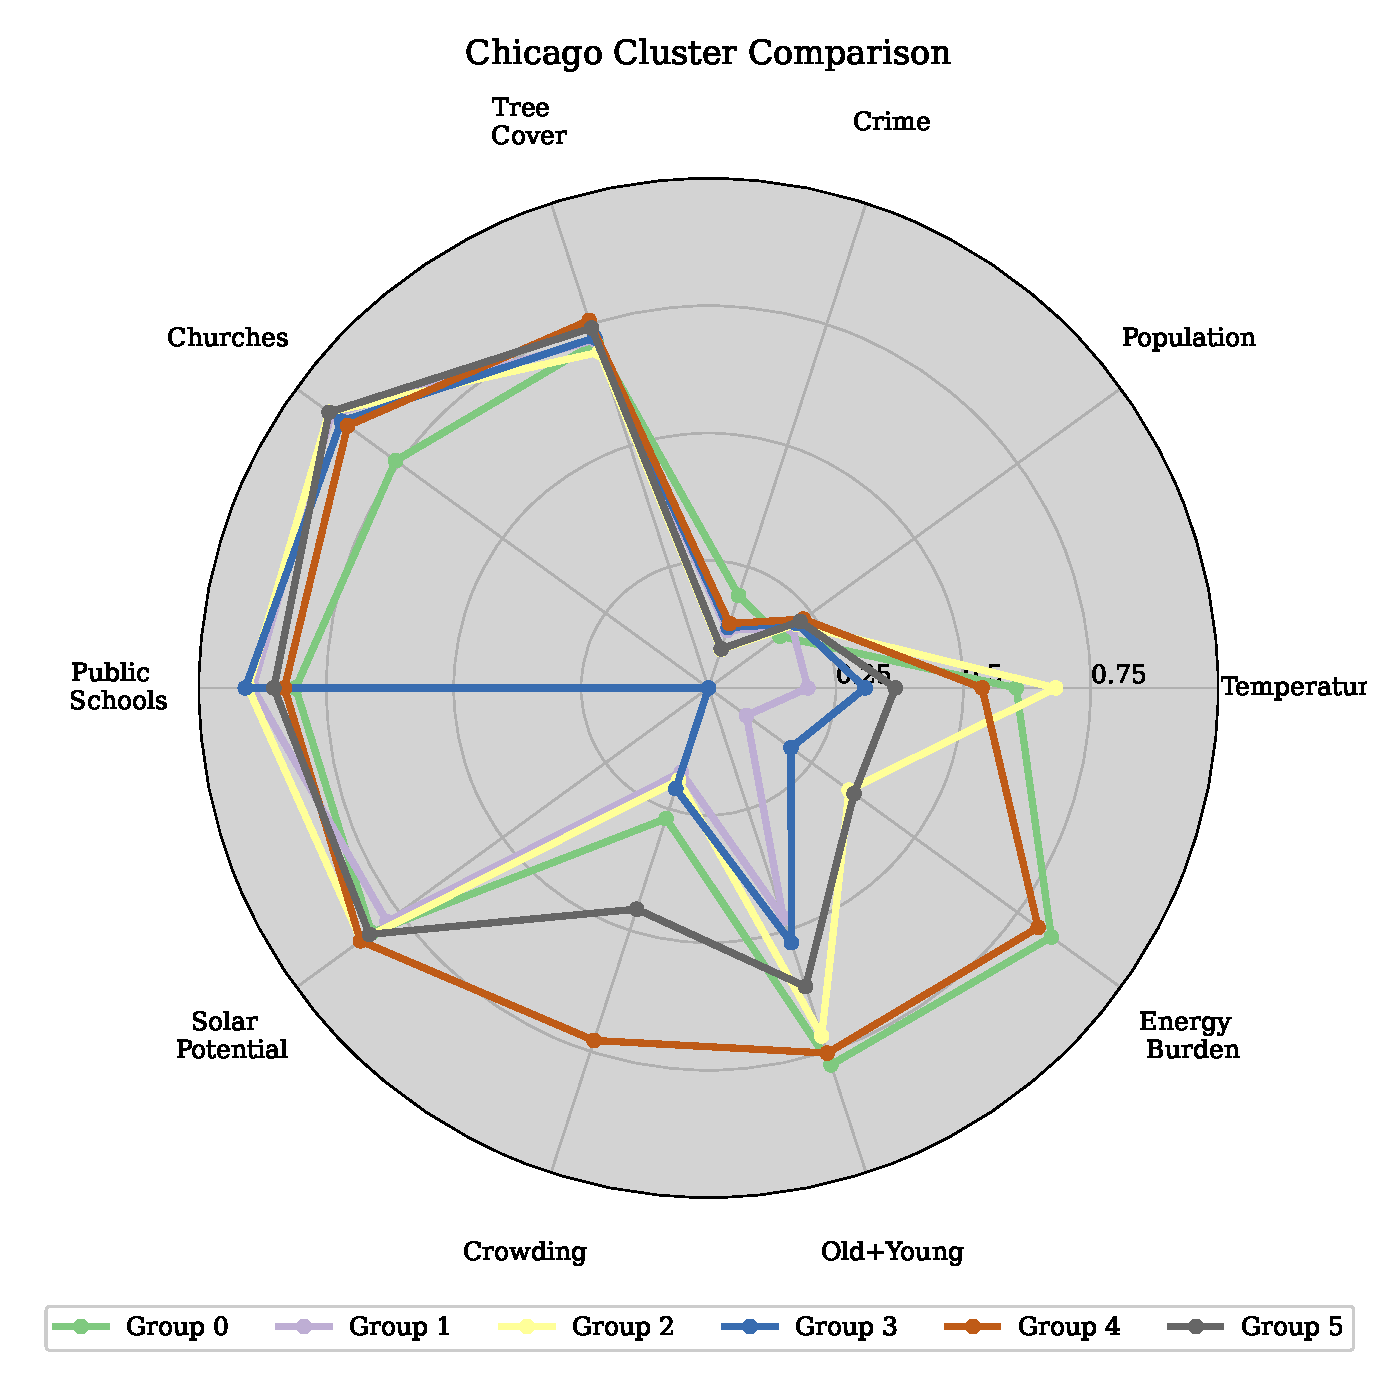
\includegraphics[width=0.95\columnwidth]{cluster_comparison}
      % \vspace*{-3cm}
      \caption{The map of Chicago clusters. The numbers correspond to the order
      in which the algorithm created the groups and not the heatwave risk.}
      \label{fig:cluster_compare}
    \end{center}
\end{figure}

There are several points of interest in Figure \ref{fig:cluster_compare}. First,
the average number of churches, public schools, crime rates, population, and tree
cover were similar across each cluster. The similarity in tree cover was unexpected
due to the strong effect of tree cover on temperature and \ac{uhi} noted in the
literature \cite{mcdonald_tree_2021,marando_urban_2022,schwaab_role_2021}. Further,
there was little difference in average crime rates across clusters. This is likely
due to the fact that a few census tracts had a much higher crime rate than all others.
With the exception of a single group, group 3, solar potential (i.e. the percent
of rooftops that qualify for solar panels \cite{google_project_2022}) was nearly
identical across all clusters.

Second, crowded housing, age, energy burden, and temperature were the most divergent
factors across the clusters. The key difference between the highest and second
highest priority clusters was crowding. It makes sense that the number of people
per household should be used to differentiate priority, \textit{ceteris paribus}.

The ``score'' that ranks the clusters is incidentally the area drawn by each
curve in Figure \ref{fig:cluster_compare}. The rank of each cluster is shown in
Figure \ref{fig:cluster_priority}.

\begin{figure}[H]
    \begin{center}
      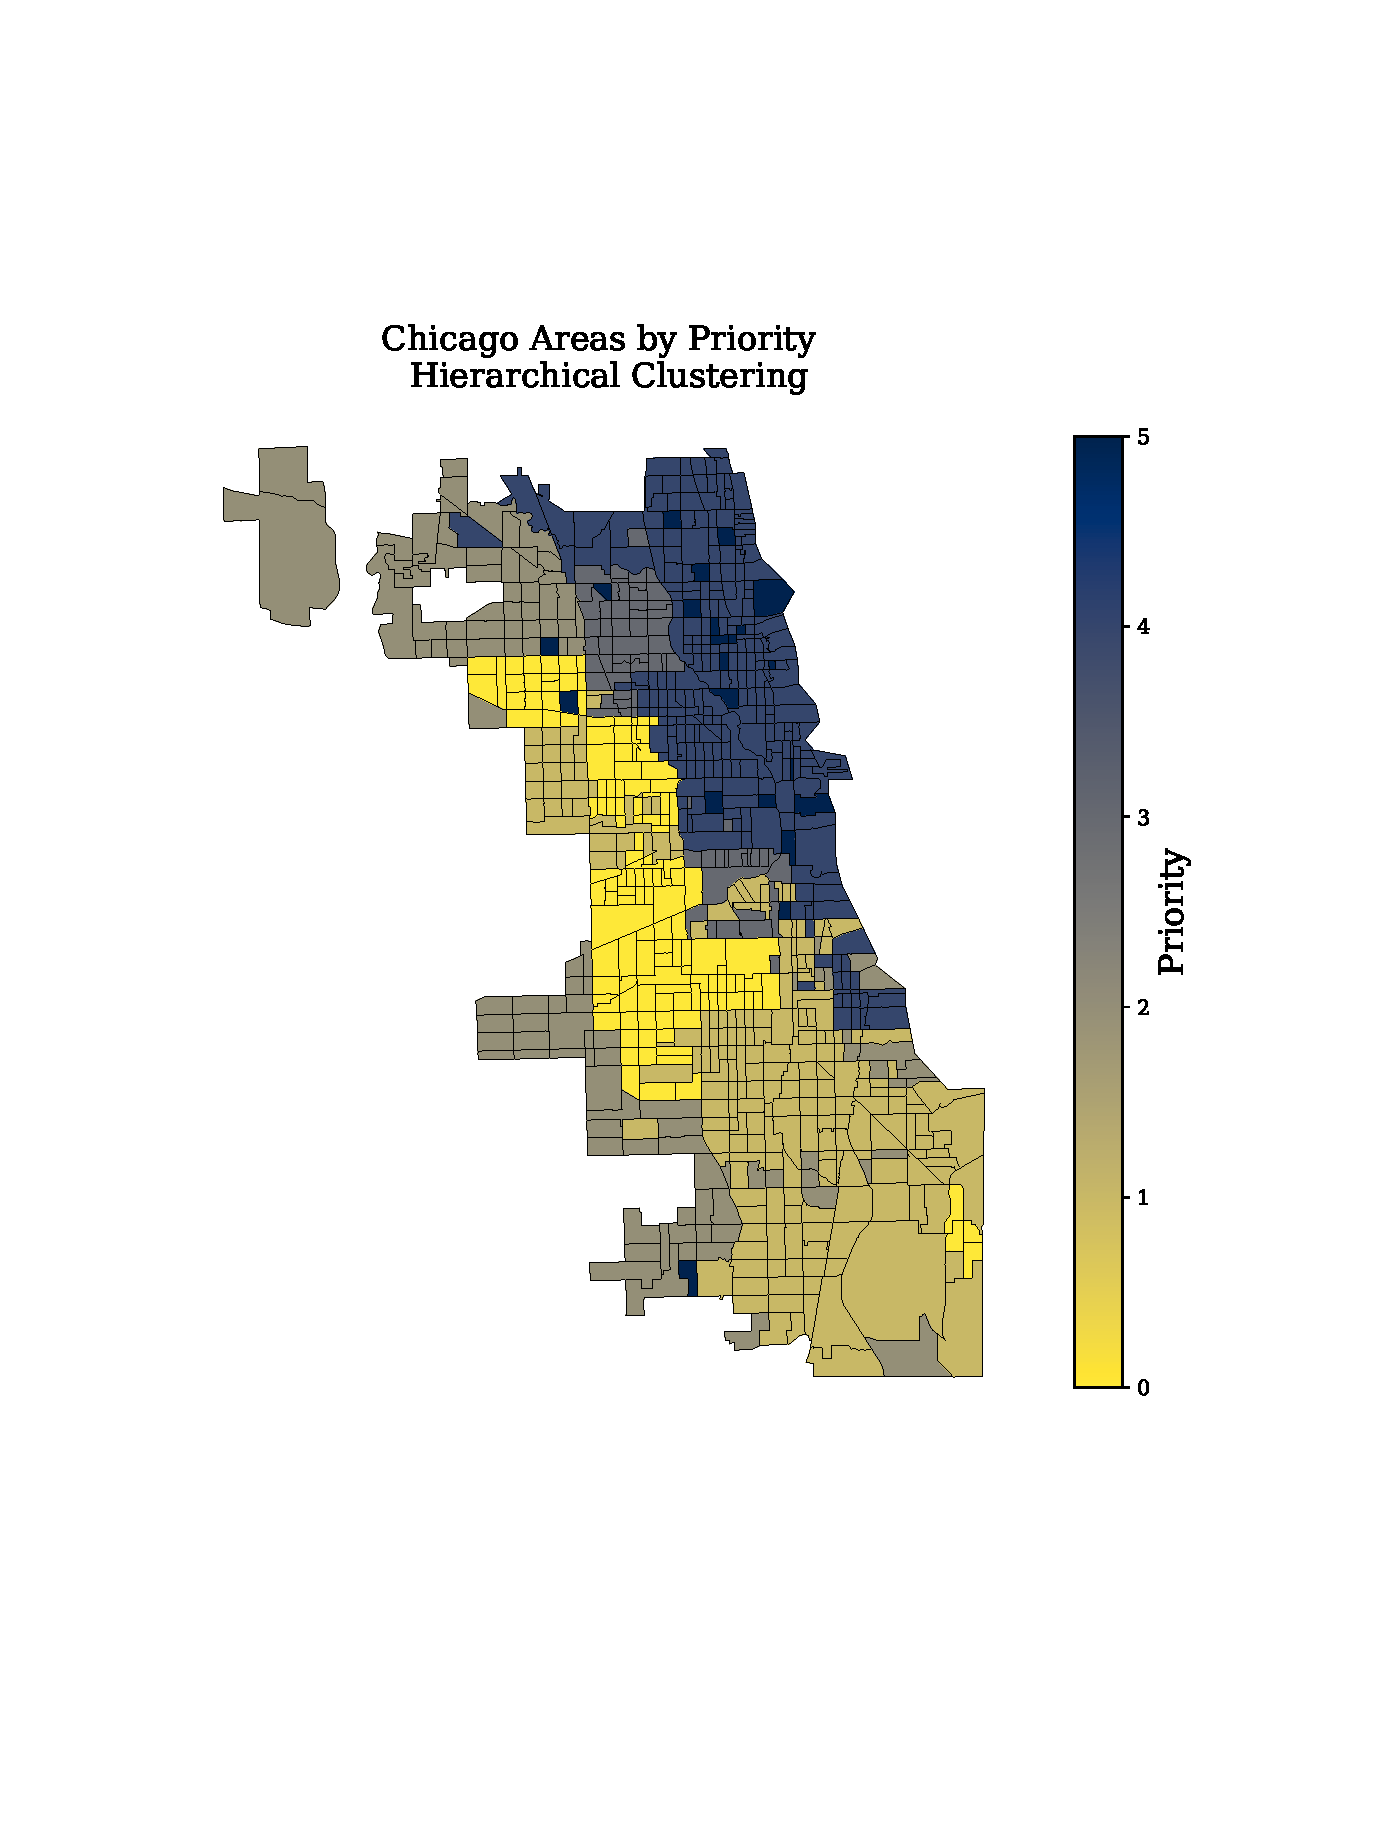
\includegraphics[trim=0 200 0 120, clip, width=\columnwidth]{clustering_priority}
      % \vspace*{-3cm}
      \caption{The map of Chicago clusters according to priority.
      0 = Highest priority. 5 = Lowest priority.}
      \label{fig:cluster_priority}
    \end{center}
\end{figure}

The highest priority region (priority 0) are on the west side of the city, where
it is warmer, crowded, and energy burden is high. The areas closest to Lake Michigan
tend to be the coolest part of the city and the most affluent, thus making them
the lowest priority (priority 5) for rooftop solar panels.

\section{Discussion}
\label{section:discussion}
The prioritization mapping protocol outlined by this research is better suited for
identifying regions for targeted incentive distribution to address specific issues
in urban settings than existing general environmental justice community
identification tools currently used for funding dissemination.

\subsection{Comparison to other Energy Justice Mapping Tools}
Other screening tools have been developed to analyze spatial characteristics of
environmental justice. The \ac{ejscreen} tool from the \ac{epa} \cite{us_epa_ejscreen_2014}
and the US Council on Environmental Quality’s \ac{cejst} tool can both be used to
identify disadvantaged or vulnerable populations spatially
\cite{council_on_environmental_quality_climate_nodate}. However, the map generated
by this research identifies a more precise region of the city of Chicago to be
prioritized for rooftop solar initiatives, therefore informing more efficient
allocation of resources to the most vulnerable communities for this particular issue.
Figure \ref{fig:ejscreen_map} and Figure \ref{fig:cejst_map} show the at-risk areas
in Chicago identified by \ac{ejscreen} and \ac{cejst}, respectively.
\begin{figure}[H]
    \begin{center}
      \includegraphics[trim=0 200 0 120, clip, width=\columnwidth]{ejscreen_map}
      % \vspace*{-3cm}
      \caption{Environmental justice communities identified by \ac{ejscreen}. ``Yes''
      indicates that the community has environmental justice concerns.}
      \label{fig:ejscreen_map}
    \end{center}
\end{figure}

\begin{figure}[H]
    \begin{center}
      \includegraphics[trim=0 200 0 120, clip, width=\columnwidth]{cejst_map}
      % \vspace*{-3cm}
      \caption{Normalized energy burden from the \ac{cejst} tool.}
      \label{fig:cejst_map}
    \end{center}
\end{figure}

Importantly, neither of these tools incorporate heatwave risk and use a limited
set of social features. The prioritization created in this research considers
traditional environmental justice factors, including age, income, and race, but
also incorporates urban heat island impacts, qualified roof area, access to cooling
centers, tree cover, and energy burden to more specifically interrogate spatial
distribution of heat impacts that could be mitigated through access to cleaner,
cheaper energy for cooling. This is a more holistic approach to understanding
environmental justice for the specific issue of access to affordable energy to
cool urban homes in a heat wave. While mapping the distribution of spatial
attributes of environmental justice can illuminate inequities at a multitude of
scales, this more precise issue-specific mapping could be more effective for
policy and incentive development.

\subsection{Targeted Incentive Distribution}

Illinois \ac{sfa} is a state-funded program that “promotes equitable access to
the solar economy through program incentives that help make solar more affordable
for low-income communities” \cite{illinois_solar_for_all_environmental_2022}. The
program allows low-income communities to benefit from community solar arrays and
distributed generation installations, as well as providing low-cost solar
installations to non-profit organizations and public facilities. Initial funding
for SFA was provided by Illinois' 2017 Future Energy Jobs Act, but when funds were
exhausted, talk of a “solar cliff” highlighted the uncertainty of the future of
solar incentives in the state (Lydersen, 2020). The popularity of this program
and limited funding for solar projects emphasizes the need for targeted distribution
of funds to the communities that need it most.

SFA has an explicit commitment to increasing access to solar energy among
environmental justice communities. SFA uses \ac{epa}’s \ac{ejscreen} and a
self-designation  process to identify environmental justice communities across
the state of Illinois. However, this method of identifying communities to target
for SFA incentives is based on a more general understanding of environmental
justice, and does not necessarily consider the potential impact of solar energy
to reduce the energy burden on low-income households through solar installation.
Targeted prioritization as outlined in this research could result in allocation
of limited solar incentive funds to the communities that would experience the
greatest benefit from solar installations by reducing risks associated with heatwaves.


\section{Conclusion}
Effective analysis of environmental justice concerns should be location-specific
and issue-focused to promote the most equitable access to incentive programs and
solutions. The argument advanced in this work is that prioritizing the distribution of solar
panels offered by programs like Solar for All or Illinois Shines will minimize the
overall heat-related adversity. Current standards for prioritizing beneficiaries
of these programs do not account for climate hazards such as heatwaves nor the
many vulnerabilities that, together, create a holistic understanding of risk.
Through this spatial analysis framework, we propose more targeted
analysis of priority beyond common methods of identifying environmental justice
communities for future allocation of solar incentive funding. This strategy could
be applied to urban environments to create a priority investment list to make
progress toward a more just energy transition nationwide.


% \bibliography
\section*{References}
\bibliographystyle{myunsrt}
\bibliography{bibliography_software}

 \end{document}
